\documentclass{emulateapj}
\submitted{{\it Submitted for publication in ApJ}}
\usepackage{multirow,color,wrapfig,ulem}
\usepackage {graphicx}
\usepackage{graphics}
\usepackage[dvips]{epsfig}

%=========================================================================
%		INTERNAL MACROS
%=========================================================================
\def\be{\begin{equation}}
\def\ee{\end{equation}}
\def\ba{\begin{eqnarray}}
\def\ea{\end{eqnarray}}

% To highlight comments 
\definecolor{red}{rgb}{1,0.0,0.0}
\newcommand{\red}{\color{red}}
\definecolor{darkgreen}{rgb}{0.0,0.5,0.0}
\newcommand{\SRK}[1]{\textcolor{darkgreen}{\bf SRK: \textit{#1}}}
\newcommand{\SRKED}[1]{\textcolor{darkgreen}{\bf #1}}
\newcommand{\before}[1]{\textcolor{red}{ #1}}
\newcommand{\after}[1]{\textcolor{darkgreen}{ #1}}

\newcommand{\LCDM}{$\Lambda$CDM~}
\newcommand{\beq}{\begin{eqnarray}}  
\newcommand{\eeq}{\end{eqnarray}}  
\newcommand{\zz}{$z\sim 3$} 
\newcommand{\avg}[1]{\langle{#1}\rangle}  
\newcommand{\ly}{{\ifmmode{{\rm Ly}\alpha}\else{Ly$\alpha$}\fi}}
\newcommand{\hMpc}{{\ifmmode{h^{-1}{\rm Mpc}}\else{$h^{-1}$Mpc}\fi}}  
\newcommand{\hGpc}{{\ifmmode{h^{-1}{\rm Gpc}}\else{$h^{-1}$Gpc}\fi}}  
\newcommand{\hmpc}{{\ifmmode{h^{-1}{\rm Mpc}}\else{$h^{-1}$Mpc}\fi}}  
\newcommand{\hkpc}{{\ifmmode{h^{-1}{\rm kpc}}\else{$h^{-1}$kpc}\fi}}  
\newcommand{\hMsun}{{\ifmmode{h^{-1}{\rm {M_{\odot}}}}\else{$h^{-1}{\rm{M_{\odot}}}$}\fi}}  
\newcommand{\Mmin}{{\ifmmode{{M_{\rm min}}}\else{${M_{\rm min}}$}\fi}}
\newcommand{\mmin}{{\ifmmode{{M_{\rm min}}}\else{${M_{\rm min}}$}\fi}}
\newcommand{\mmax}{{\ifmmode{{M_{\rm max}}}\else{${M_{\rm max}}$}\fi}}
\newcommand{\lmmin}{{\ifmmode{{\log M_{\rm min}}}\else{${\log M_{\rm min}}$}\fi}}
\newcommand{\lmmax}{{\ifmmode{{\log M_{\rm max}}}\else{${\log M_{\rm max}}$}\fi}}

\newcommand{\Mmax}{{\ifmmode{{M_{\rm max}}}\else{${M_{\rm max}}$}\fi}}
\newcommand{\dm}{{\ifmmode{{\Delta M}}\else{$\Delta M$}\fi}}
\newcommand{\dlm}{{\ifmmode{{\Delta \log M}}\else{$\Delta \log M$}\fi}}
\newcommand{\focc}{{\ifmmode{{f_{\rm occ}}}\else{${f_{\rm occ}}$}\fi}}

\newcommand{\Msun}{{\ifmmode{{\rm {M_{\odot}}}}\else{${\rm{M_{\odot}}}$}\fi}}  
\newcommand{\msun}{{\ifmmode{{\rm {M_{\odot}}}}\else{${\rm{M_{\odot}}}$}\fi}}  
\newcommand{\lya}{{Lyman$\alpha$~}}
\newcommand{\clara}{{\texttt{CLARA}}~}
\newcommand{\rand}{{\ifmmode{{\mathcal{R}}}\else{${\mathcal{R}}$ }\fi}}  
%SAMPLES


%MY COMMANDS #############################################################
\newcommand{\sub}[1]{\mbox{\scriptsize{#1}}}
\newcommand{\dtot}[2]{ \frac{ d #1 }{d #2} }
\newcommand{\dpar}[2]{ \frac{ \partial #1 }{\partial #2} }
\newcommand{\pr}[1]{ \left( #1 \right) }
\newcommand{\corc}[1]{ \left[ #1 \right] }
\newcommand{\lla}[1]{ \left\{ #1 \right\} }
\newcommand{\bds}[1]{\boldsymbol{ #1 }}
\newcommand{\oiint}{\displaystyle\bigcirc\!\!\!\!\!\!\!\!\int\!\!\!\!\!\int}
\newcommand{\mathsize}[2]{\mbox{\fontsize{#1}{#1}\selectfont $#2$}}
\newcommand{\eq}[2]{\begin{equation} \label{eq:#1} #2 \end{equation}}
\newcommand{\lth}{$\lambda_{th}$ }
\newcommand{\reff}{{\ifmmode{r_{\mbox{\tiny eff}}}\else{$r_{\mbox{\tiny eff}}$}\fi}}
%#########################################################################

%TO DO COMMANDS. Highlight region that needs extra work  #############################################################
\newcommand{\todo}{\ifmmode \text{\Huge{\(\bullet\)}} \else {\Huge$\bullet$}\fi}
% \newcommand{\todo}{\ifmmode {\Huge \bullet} \else {\Huge$\bullet$}\fi}
\newcommand{\tido}{\ifmmode {\bullet} \else $\bullet$\fi}
\newcommand{\REFS}{(\todo REFS) }
\newcommand{\toref}{(\todo REFS)}
%#########################################################################



\begin{document}
%=========================================================================
%		FRONT MATTER
%=========================================================================
\title{Satellite Alignments in Galaxy Pairs}
\author{
  Ver\'onica Arias \thanks{v.arias@uniandes.edu.co}$^{1}$,
  Jaime E. Forero-Romero \thanks{je.forero@uniandes.edu.co}$^{2}$ 
}

\affil{
$^1$Departamento de F\'{i}sica, Universidad de los Andes, Cra. 1
No. 18A-10, Edificio Ip, Bogot\'a, Colombia\\
}




\begin{abstract}
Alineaciones.
\end{abstract}

\keywords{
Galaxies: halos --- Galaxies: high-redshift --- Galaxies: statistics
--- Dark Matter --- Methods: numerical 
}

\section{Introduction}

%
%Observational evidence of planes is everywhere (where we can see them). MW, M31, Centaurus A.\\
%
%Not so evident in simulations:\\
%
%Millenium II Baumgardt, Ibata, Pawlowski\\
%
%Clues Gillet está pero diferente\\
%
%Plane claims:\\
%Libeskind: preferential direction for accretion.\\
%Sawala: planes are there when baryonic physics is included.\\
%Buck: planes are easy to form at early times, when DM filaments are very thin. In high redshift galaxies galaxies, planes are everywhere.\\
%
%Other explanations: Kroupa: tidal dwarfs\\
%Fouquet\\
%
%
%
% 
%Following a bit on the claim by Sawala that barionic physics are important when looking for planes, WE look in Illustris and Elvis simulations to try and understand why barionic physics results in planar distribution of satellites.

%\subsection{Evidencias observacionales de planos:}
\noindent Since the early works of (el que libeskind dice que habló de
eso primero) and Lynden-Bell (1976), the observed anisotropic
distribution of satellite galaxies in the Local Group has been a key
point in the discussion of galaxy formation models within $\Lambda$CDM
cosmology. These pioneer papers described that the then known satellite
galaxies of the Milky May (MW) were distributed roughly following the plane
that contained the Magelanic clouds and their stellar tails. This
anisotropic distribution was further studied in the work of Pawlowski
et. al. (2012), where they included all the known MW satellite galaxies (XXX
more than in the original Lynden-Bell paper) as well as some MW globular
clusters, and found that they are all contained in what they call a
"Vast Plane Of Satellites" (VPOS). This structure is around 30kpc thick and
is perpendicular to the stellar disc of the MW galaxy. This plane of
satellites was considered a rarity until the PAndAS survey of the
Andromeda (M31) galaxy and its halo (missing reference on the survey)
provided a complete sample of the satellite galaxy population (above a
XXXX magnitude) of our neighboring galaxy, allowing their consistent distance
estimations (Conn et al 2012). In a groundbreaking work, Ibata et.
al. (2013) found that 15 out of the 30 satellites are in a planar
structure that is 15kpc thick and has an extension of 400kpc.
Additionally, from line of sight velocity measurements, they
found that the structure has an apparent coherent rotation, with the
satellites south of M31 moving away from us and those north of M31
coming towards us. This apparent organized rotation of satellite galaxies was also
statistically found to occur in diametrically opposed 
pairs of satellites from the SDSS (Ibata et al 2014), although this
results were contested in a follow up paper by Cuatun et al (2014).  

These discoveries of the planes in M31 and the MW were followed by the
remark from Shaya et al (2013) that the other satellite galaxies in
M31 could be part of a second plane, further reinforcing the idea that
satellites in the local group are not isotropically distributed.
Despite the challenges in estimating distances to the satellites
galaxies, Tully et al. managed to go beyond the local group and found
two planes of satellites galaxies in Centaurus A, making a clearer
case for the planes of satellites>in all the galaxies where distance
measurements could be performed evidence of satellite planar
structures have been found.\\

These observed planes present a challenge for current galaxy formation
models (Pawlowski et. al 2014)


%The VPOS (Pawlowski et al 2012: https://arxiv.org/abs/1204.5176)\\
%A vast thin plane of corrotating dwarf galaxies orbiting the Andromeda
%Galaxy (Ibata et al 2013)\\
%Corotation in SDSS data (Ibata et al 2014)\\
%There was a reply to this paper (A new spin on disks of satellite
%galaxies, Cuatun et al 2014)\\
    %Planes in Centaurus A (Tully et al 2015)\
%paper con los dos planos MW yM31
%>https://arxiv.org/pdf/1307.6210v1.pdf
\
%Varios papers de pawlowski que muestran que los nuevos sat\'elites de
%MW estan en el plano, que el plano no se debe al Sdss footprint, que
%los globular clusters tambien estan en el plano... etc,\\ 
%Papers de Conn donde encuentra el plano\\

%\subsection{B\'usqueda de planos en simulaciones:}
\noindent A comparison of the distribution of satellite galaxies
around Andromeda and the results of $\Lambda$CDM simulations (Bahl and
Baumgardt 2013) Encuentran planos en Millenium II.\\
A thousand shadows of Andromeda: rotating planes of satellites in the
Millennium-II cosmological simulation (Ibata et al 2013) dicen que el
paper de Bahl y Baumgardt est\'a mal y que no hay planos en millenium
II\\
Co-orbiting satellite galaxy structures are still in conflict with the
distribution of primordial dwarf galaxies (Pawlowski et al 2014)\\
Co-orbiting planes of sub-halos are similarly unlikely around paired
and isolated hosts (Pawlowski et al 2014)\\
Vast planes of satellites in a high resolution simulation of the Local
Group: comparison to Andromeda (Gillet et al 2014). finds a plnes
similar to that of M31 in Clues simulations.\\
Planes of satellite galaxies: when exceptions are the rule (Cautun et
al 2015) encuentra que 10 por ciento de los halos tienen planos
iguales o m\'as prominentes que los del LG.\\

\subsection{Posibles or\'igenes de los planos:}
\noindent Preferential accretion (Libeskind et al 20??)\\
Alignments with the cosmic web (Tempel et al 20??)\\
The vast thin plane of M31 co-rotating dwarfs: an additional fossil
signature of the M31 merger and of its considerable impact in the
whole Local Group (Hammer et al 2013) Major merger in M31-MW system
plane galaxies are tidal dwarfs (n-body simulations)\\
Kroupa tiene todo un carretazo de que las dwarfs son todas tidal
dwarfs\\
MIRAR lo que est\'a haciendo Pierre Alan Duc con tidal dwrafs porque en
una conferencia este a;o habl\'o de un posible escenario
intermedio...\\
Evidence for Early Filamentary Accretion from the Andromeda Galaxy's
Thin Plane of Satellites (Buck et al 2015)\\
Alignments between galaxies, satellite systems and haloes (Cautun et al
2016) NO LO HE LEIDO...

\subsection{Problemas con esas explicaciones:}
The Vast Polar Structure of the Milky Way and Filamentary Accretion of
Sub-Halos (Pawlowski et al 2012)\\
Paper de Collins (2013 y 2016) donde explica que no hay doferencias en
las propiedades de los on-plane y los off-plane satellites\\
Problemas con la estabilidad a largo plazo de los planos: Bowden et al
2012, Gonzales et al 2015...\\
The Plane Truth: Andromeda analog thin Planes of Satellites are not
kinematical coherent structures (Buck et al 2015)\\


\section{Illustris simulation}

\section{Sample Selection}

General Pair Sample.

Reduced sample based on non interacting halos. Further sub-selection based on number of bright substructures.

Reduced Local Group sample based on kinematic characteristics.

\begin{figure}
\centering
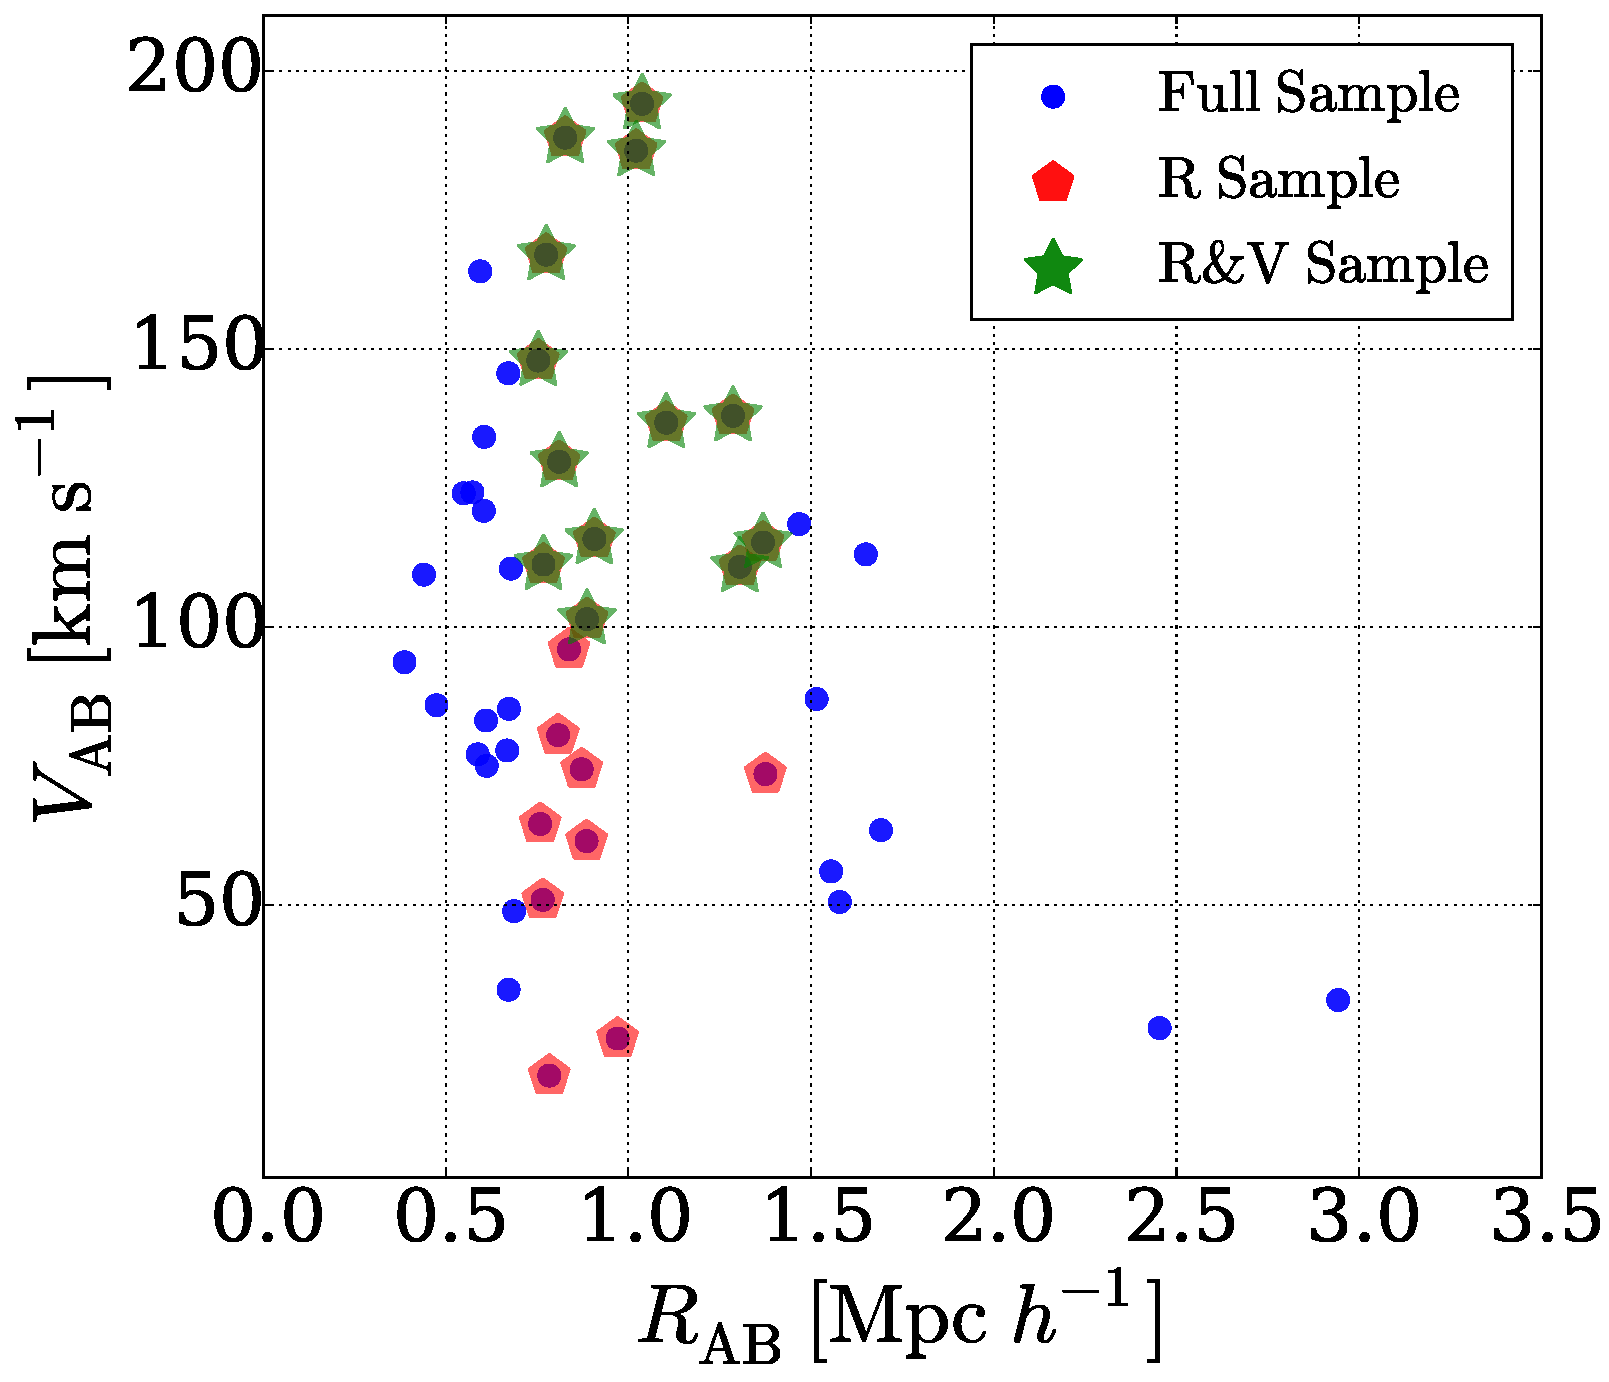
\includegraphics[width=\hsize]{v_r_pairs.pdf}\\
\caption{Halo pair samples used in this paper located in the
  plane of relative comoving velocity $V_{AB}$ versus relative
  distance $R_{AB}$ between the two halos in the pair.
  The R\&V sample is the closest to the separation and kinematic
  conditions observed in the Local Group.} 
\label{fig:samples}
\end{figure}

\begin{figure}
\centering
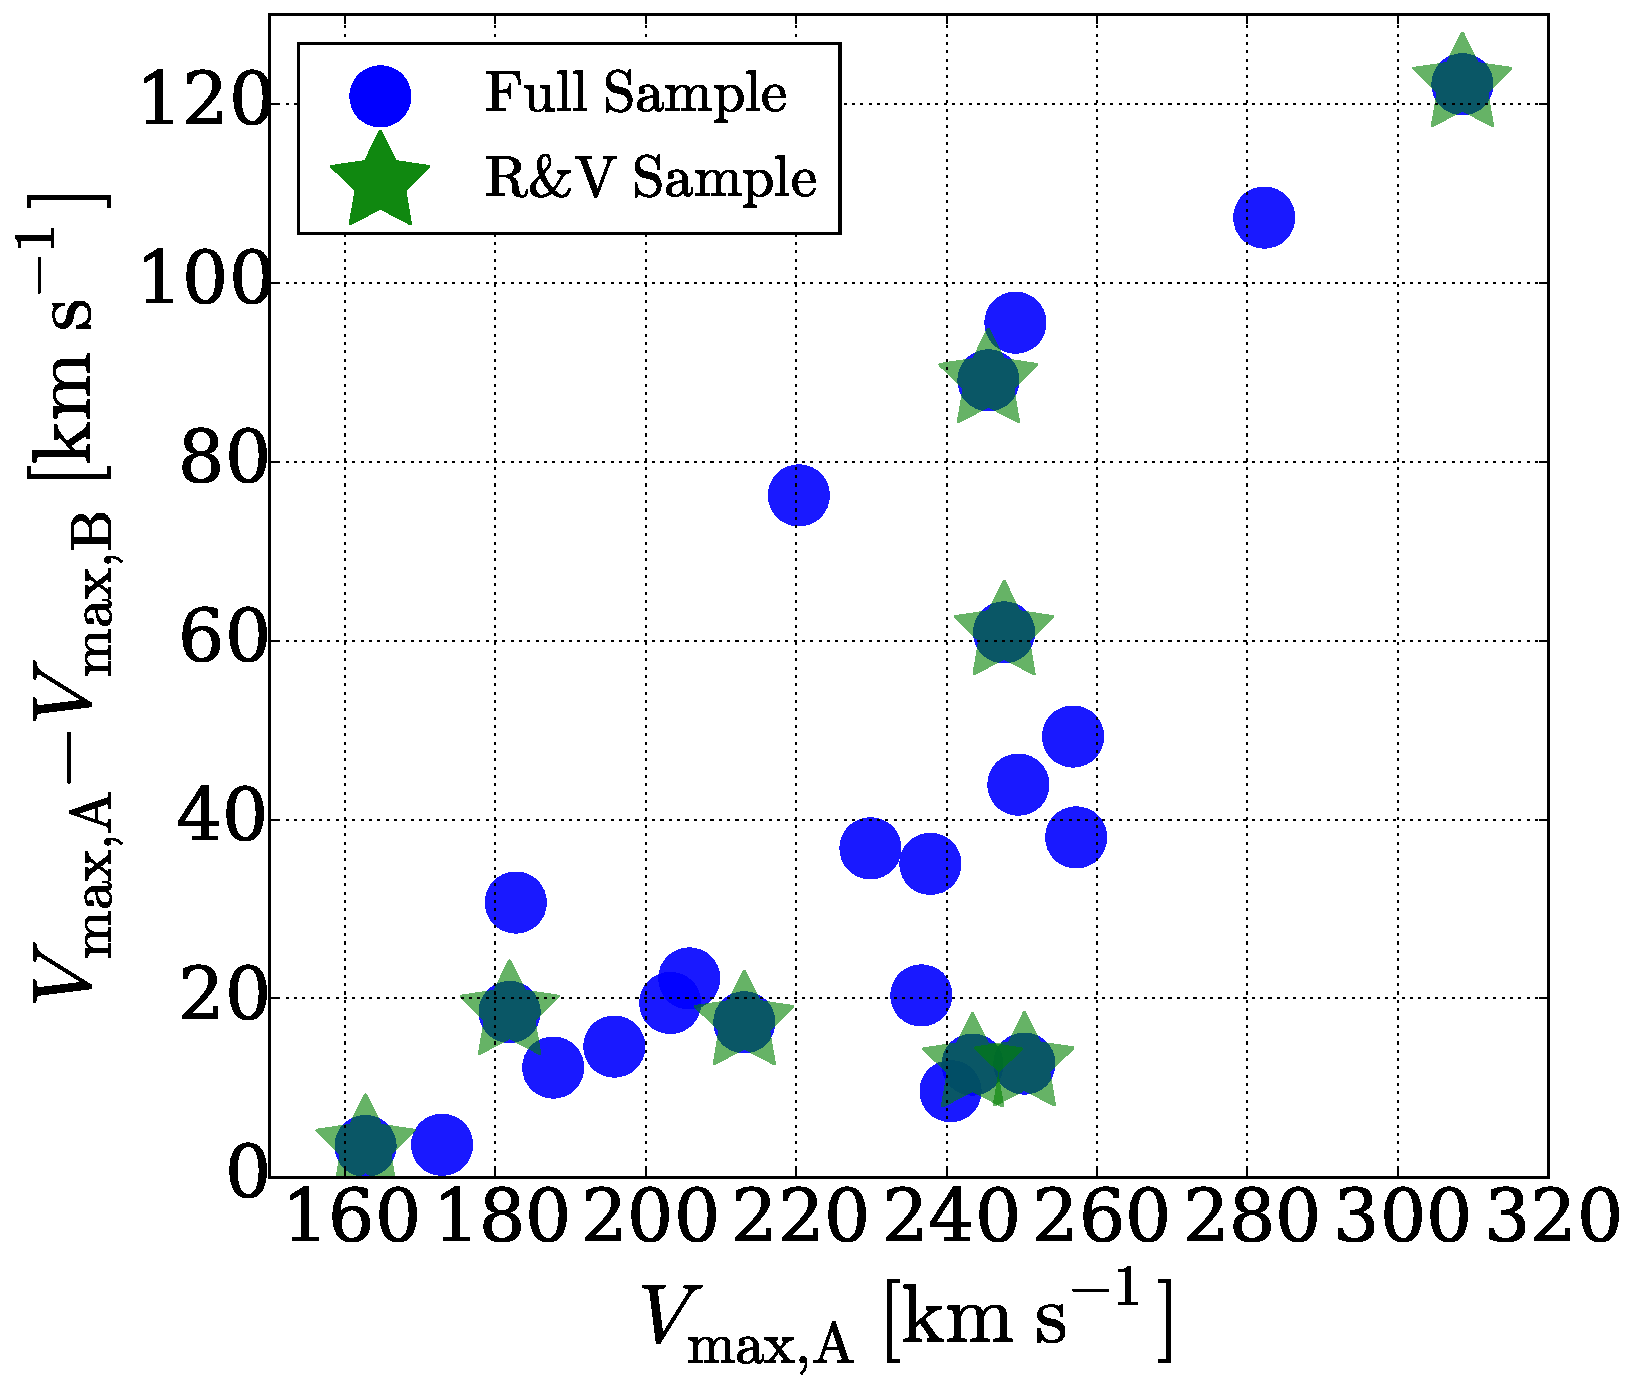
\includegraphics[width=\hsize]{v_circ_pairs.pdf}\\
\caption{Diference between the maximum circular velocity $V_{max}$ for the two
  halos in the pair as a function of $V_{max}$ for the massive halo in
  the pair.}
\label{fig:vcirc}
\end{figure}

\begin{figure}
\centering
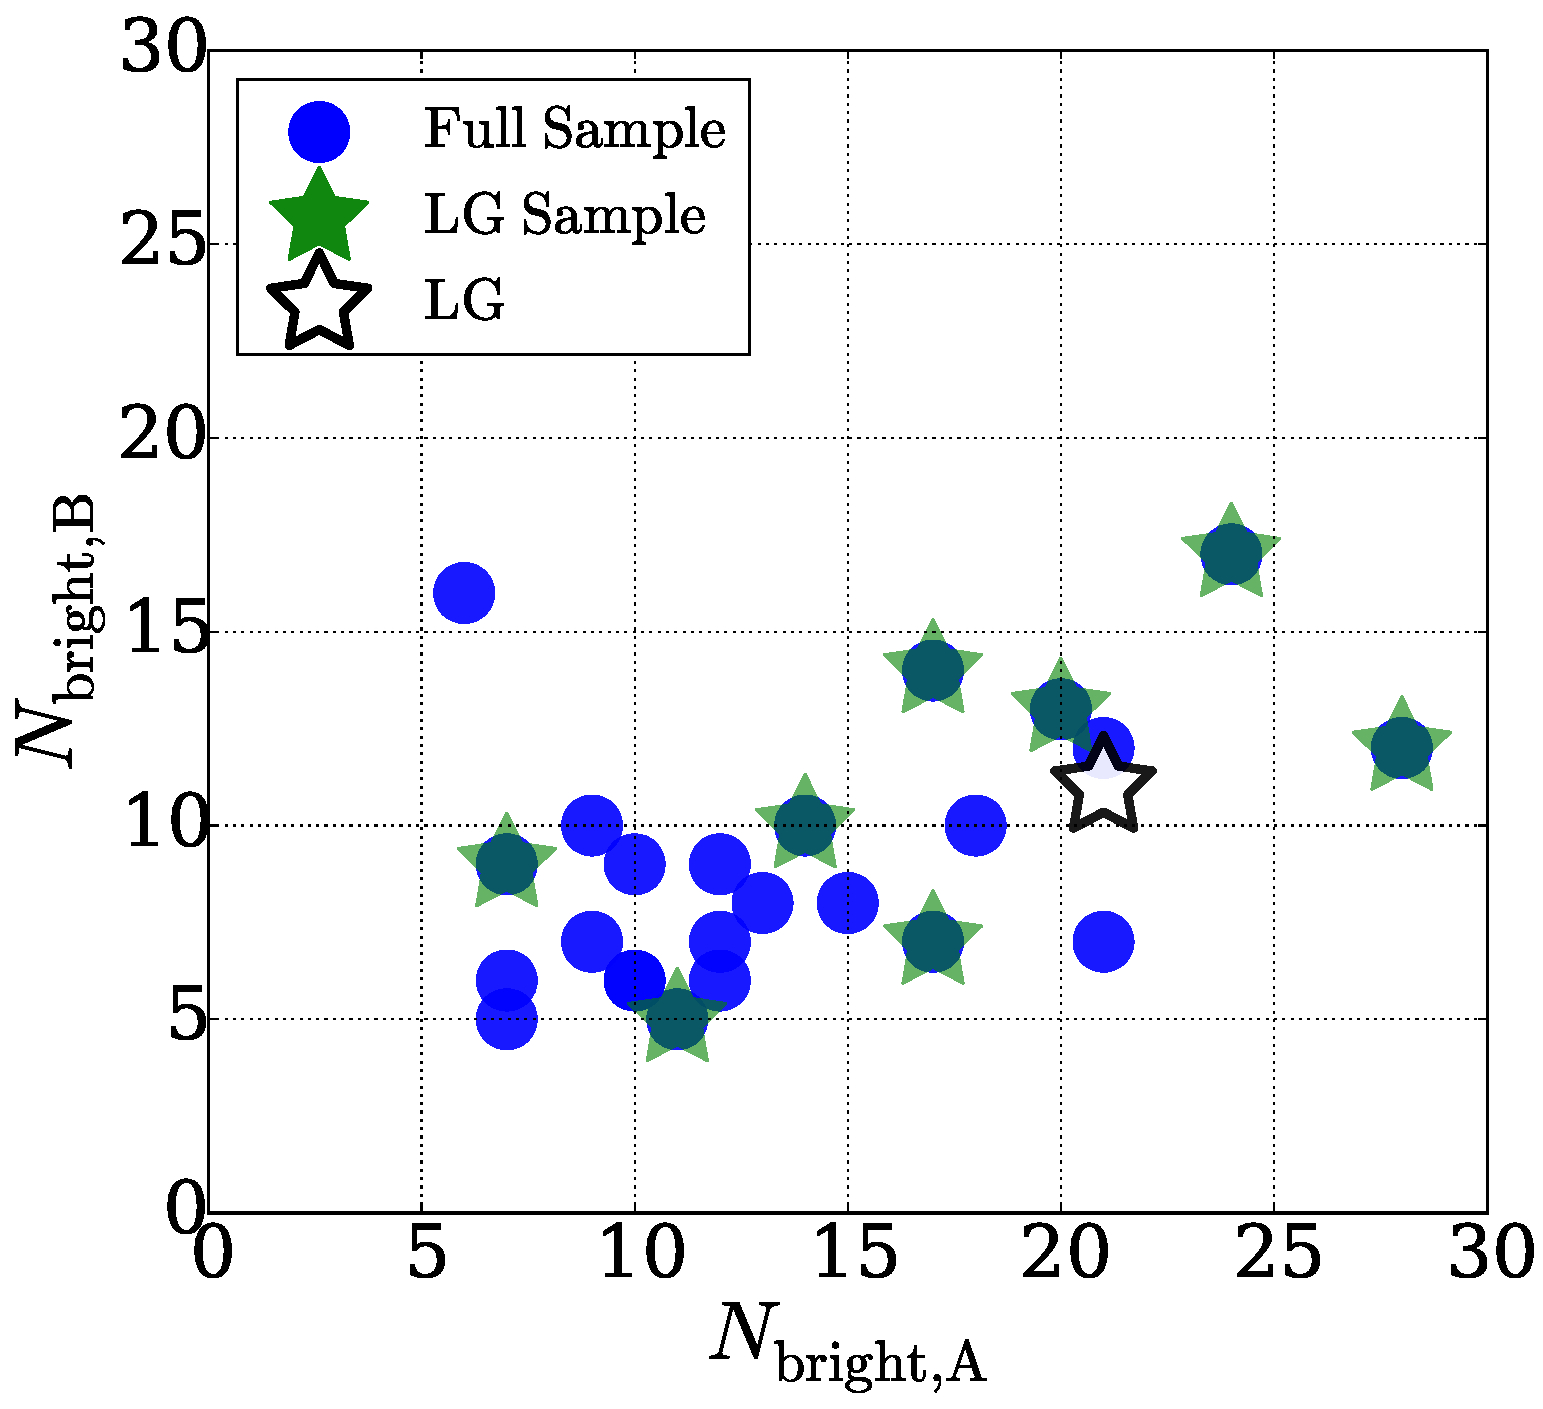
\includegraphics[width=\hsize]{n_structure.pdf}\\
\caption{Number of bright substructures ($M_{B}<-9$) and dark matter
  substructures.}
\label{fig:nstructure}
\end{figure}



\begin{figure}
\centering
\includegraphics[width=\hsize]{axratio_dark_bright.pdf}\\
\caption{Axis ratio of luminous satellites versus the axis ratio for
  dark subhalos.}
\label{fig:StreamPlaneOrbit}
\end{figure}


\begin{figure*}
\centering
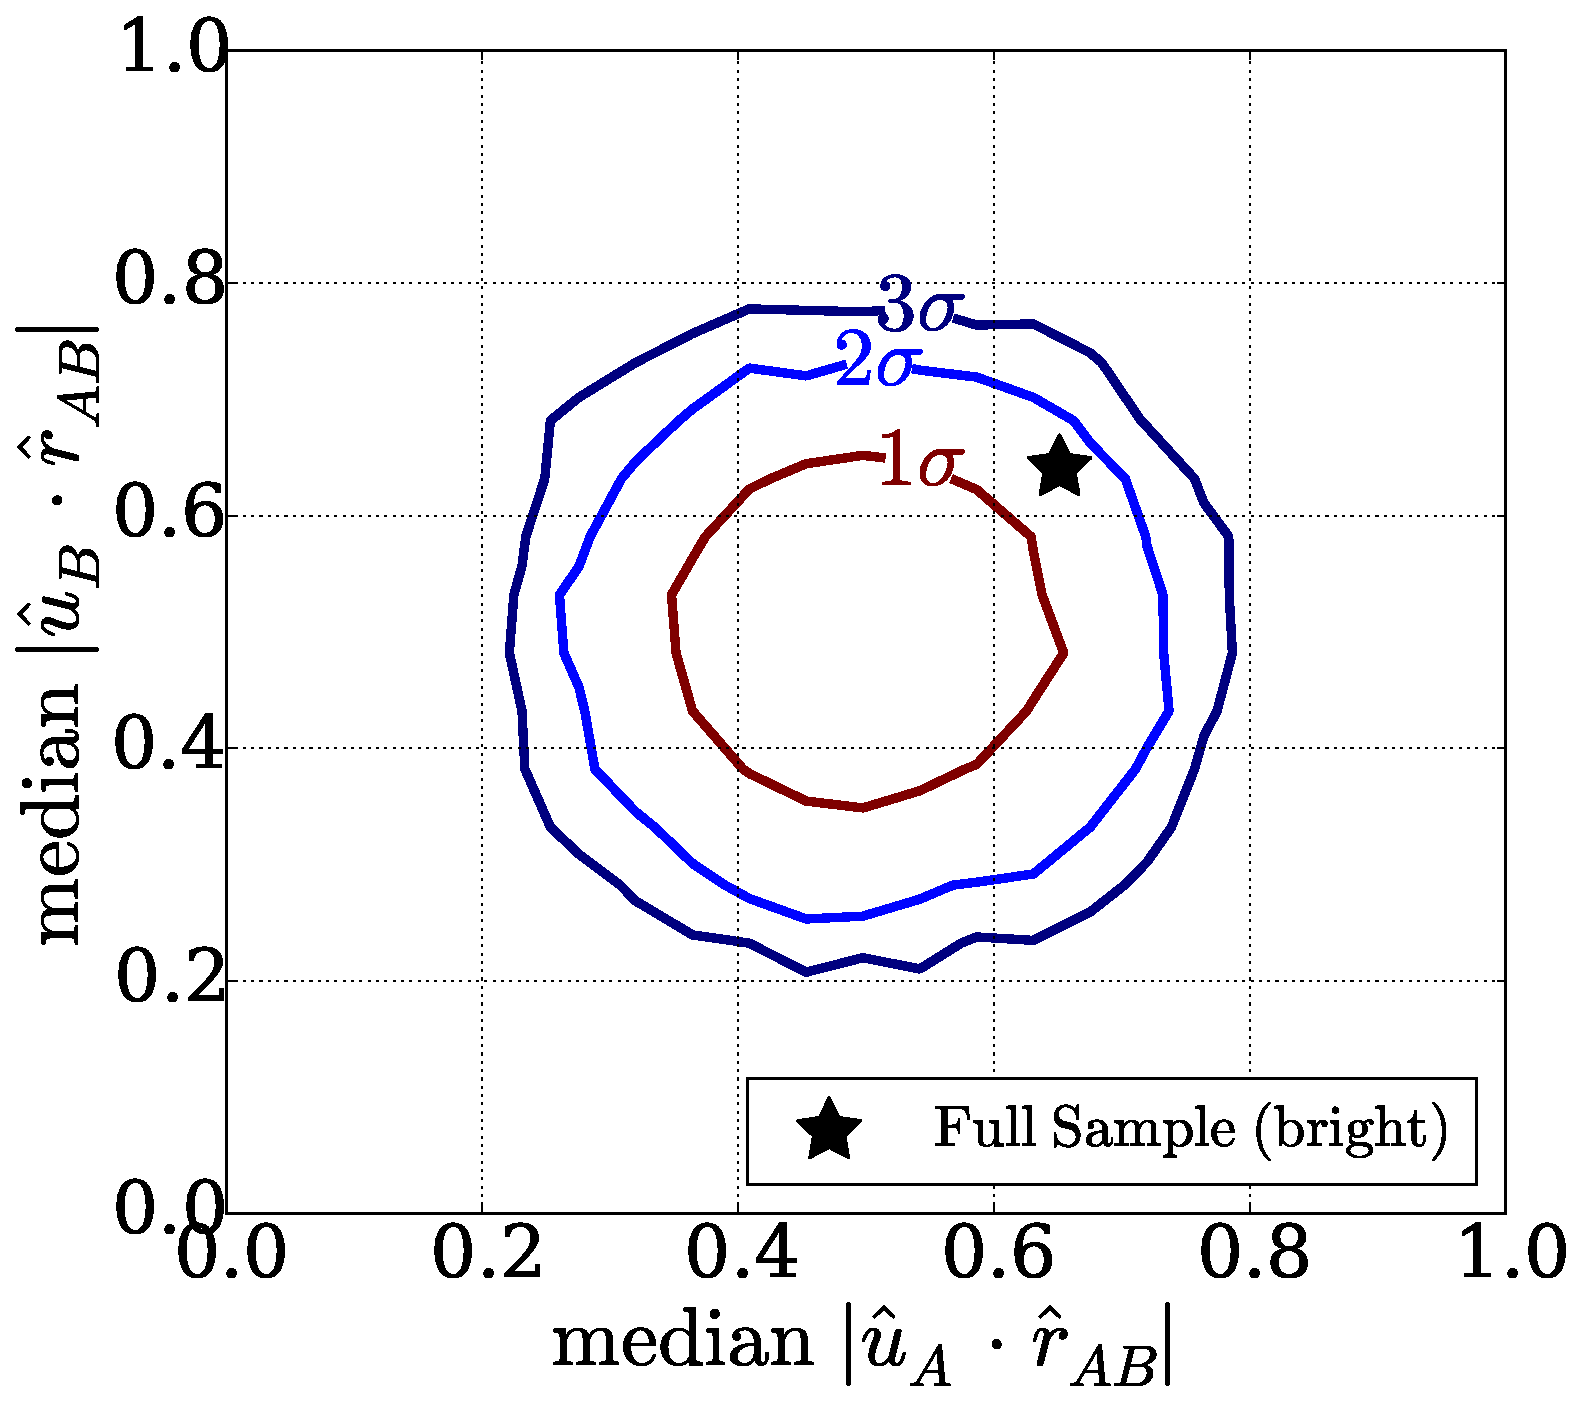
\includegraphics[width=0.48\hsize]{significance_full_bright.pdf}
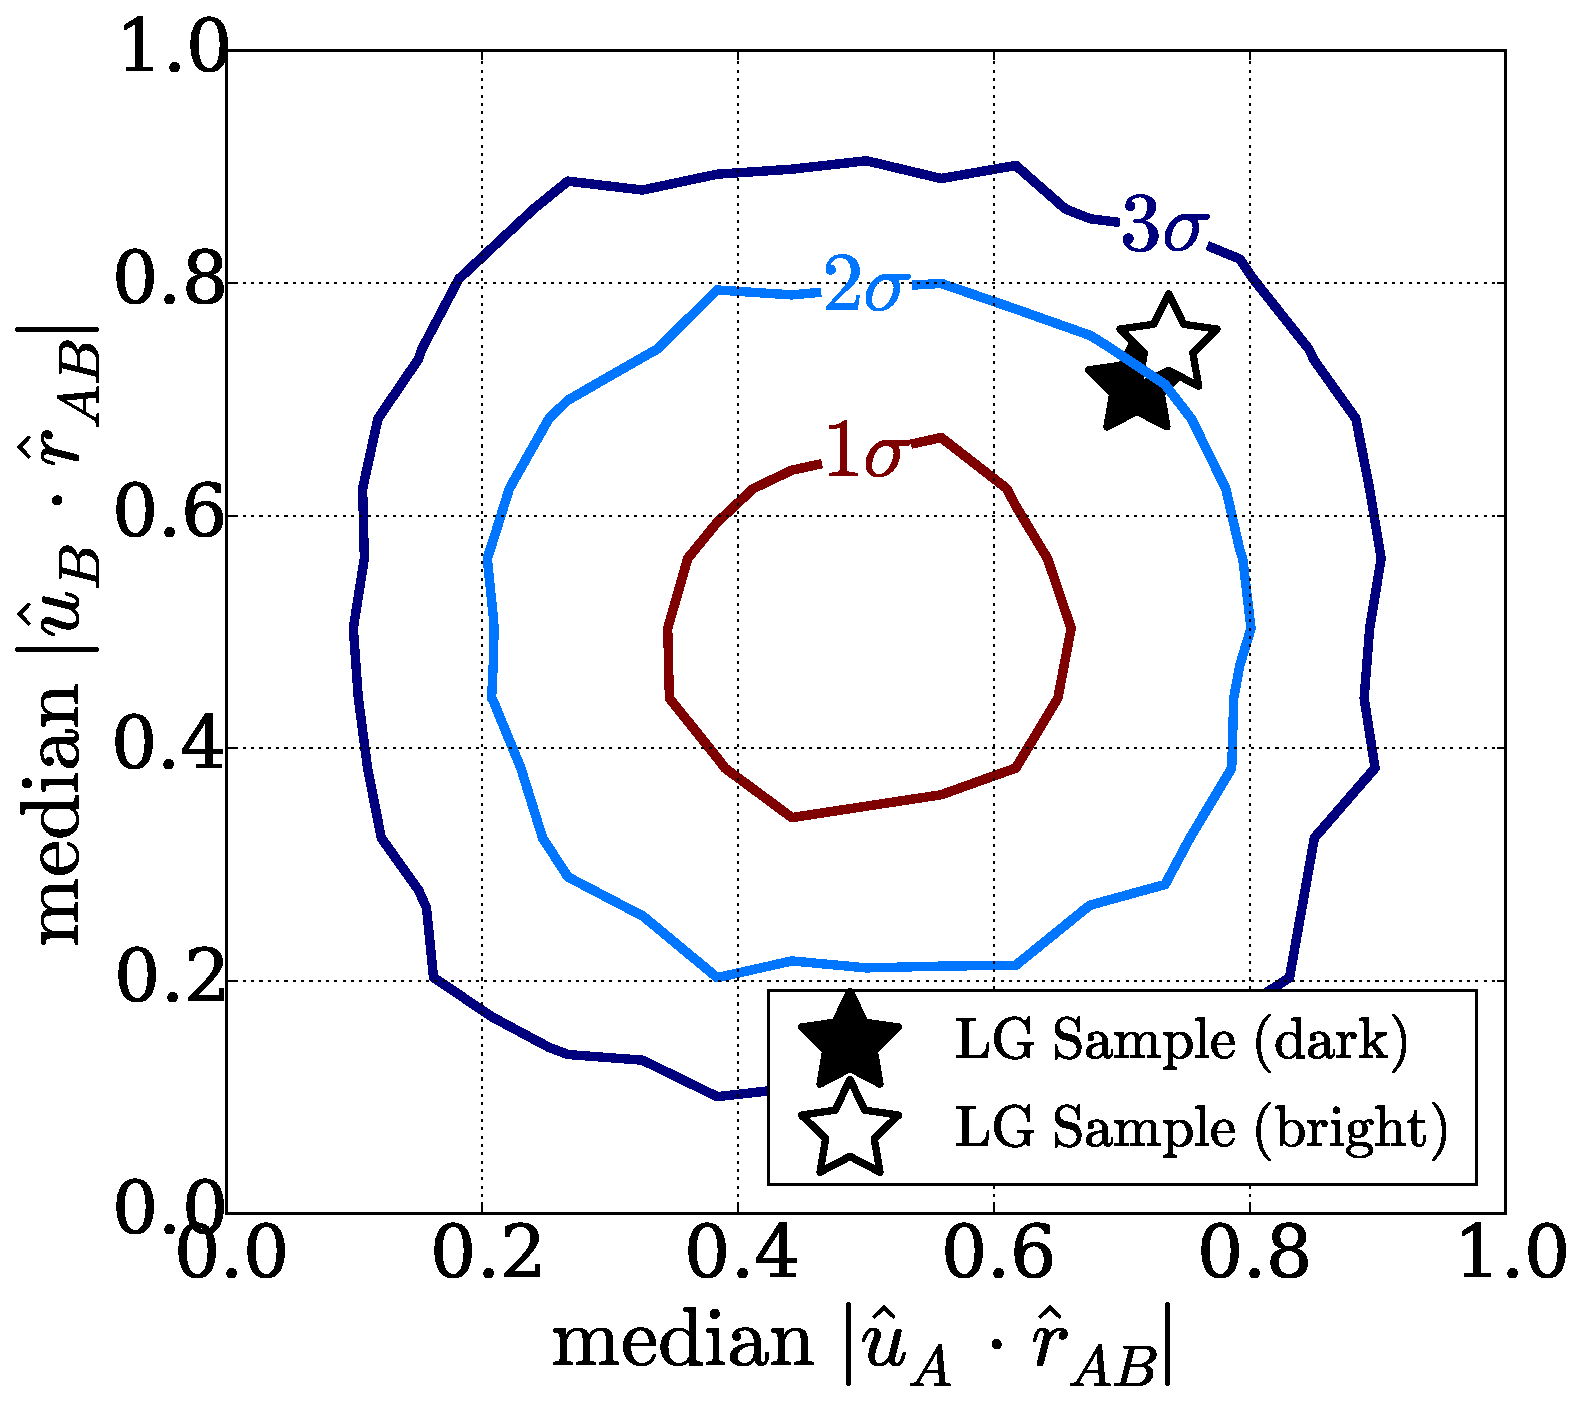
\includegraphics[width=0.48\hsize]{significance_lg_bright.pdf}
\caption{Significance of alignments.}
\label{fig:significance}
\end{figure*}

\begin{figure}
\centering
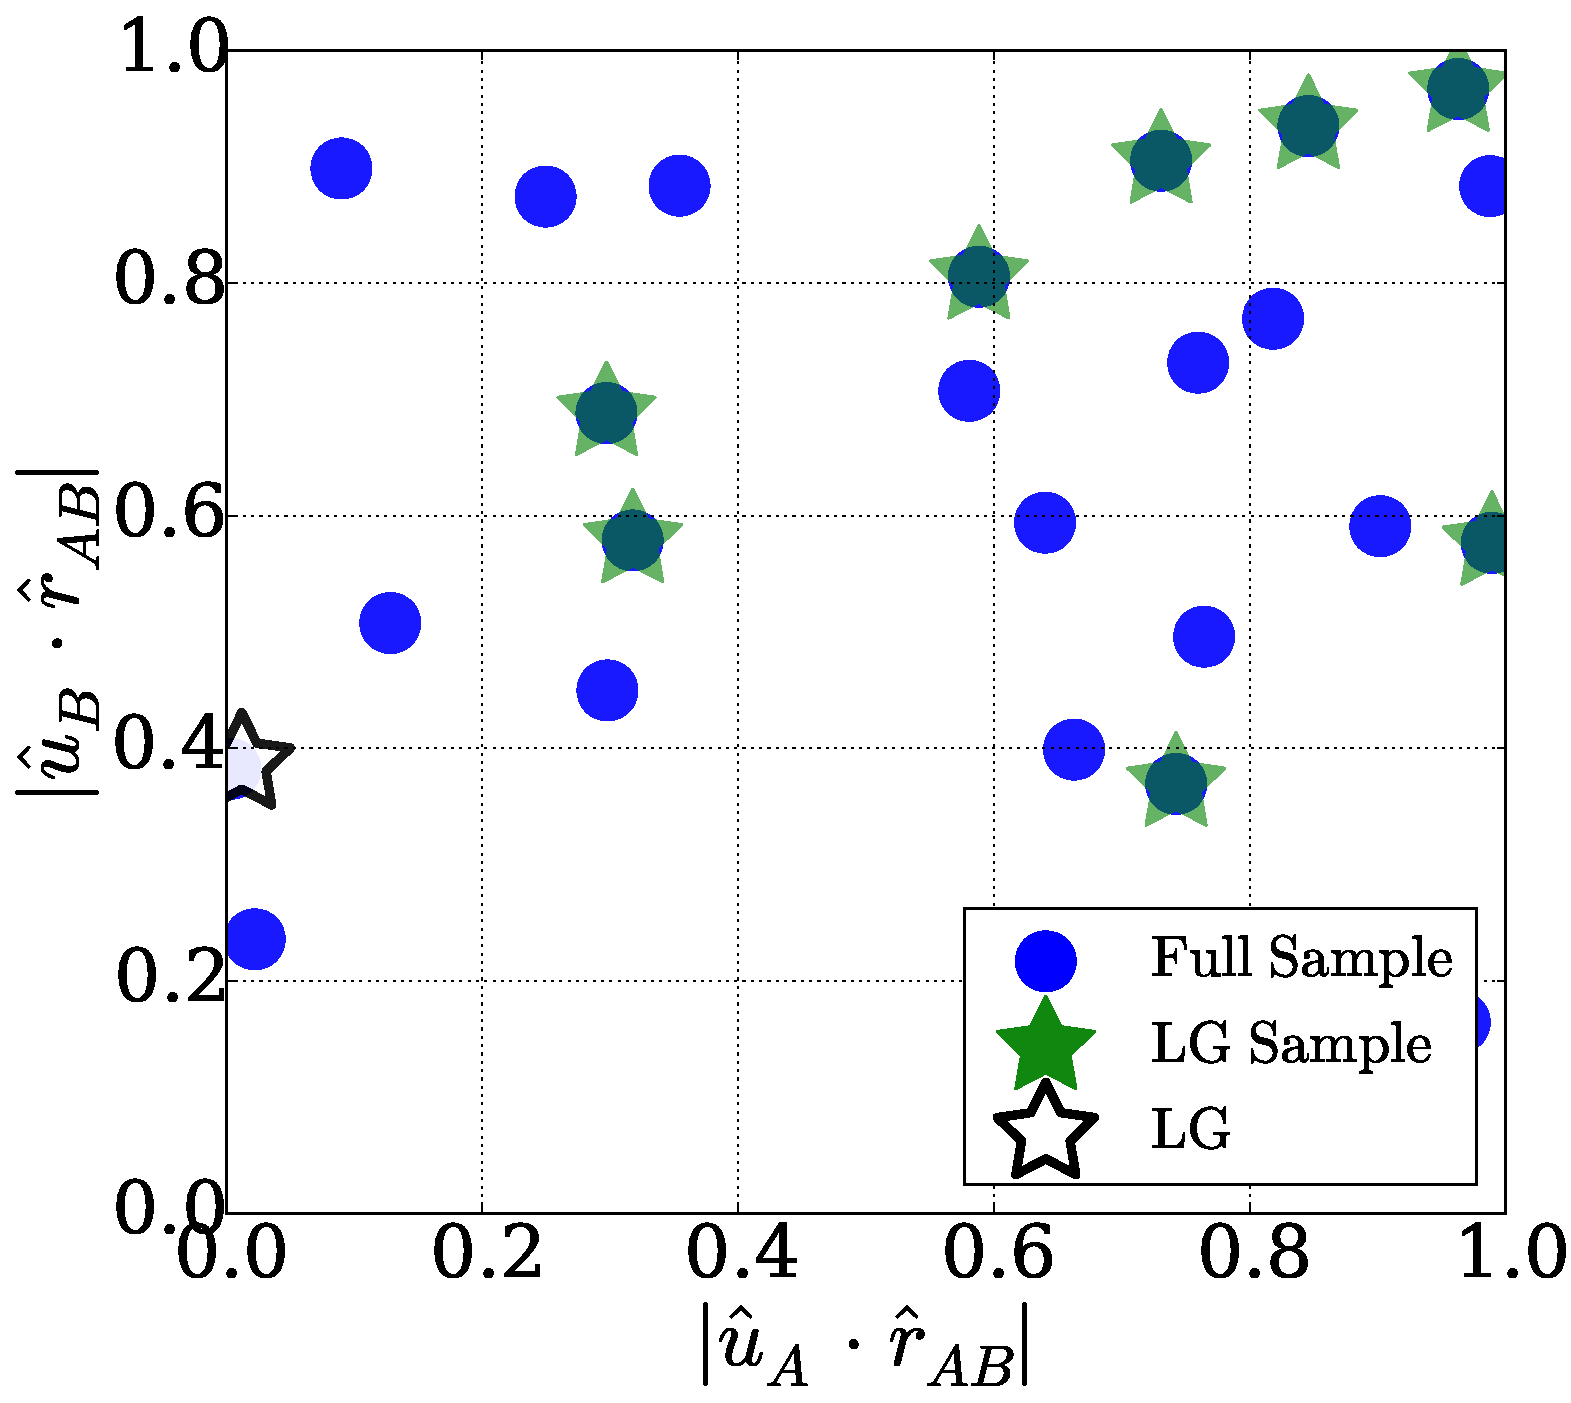
\includegraphics[width=\hsize]{r_u_alignment.pdf}\\
\caption{Alignment of the mayor axis with the vector connecting the
  two halos.}
\label{fig:lg_alignment}
\end{figure}

\begin{figure}
\centering
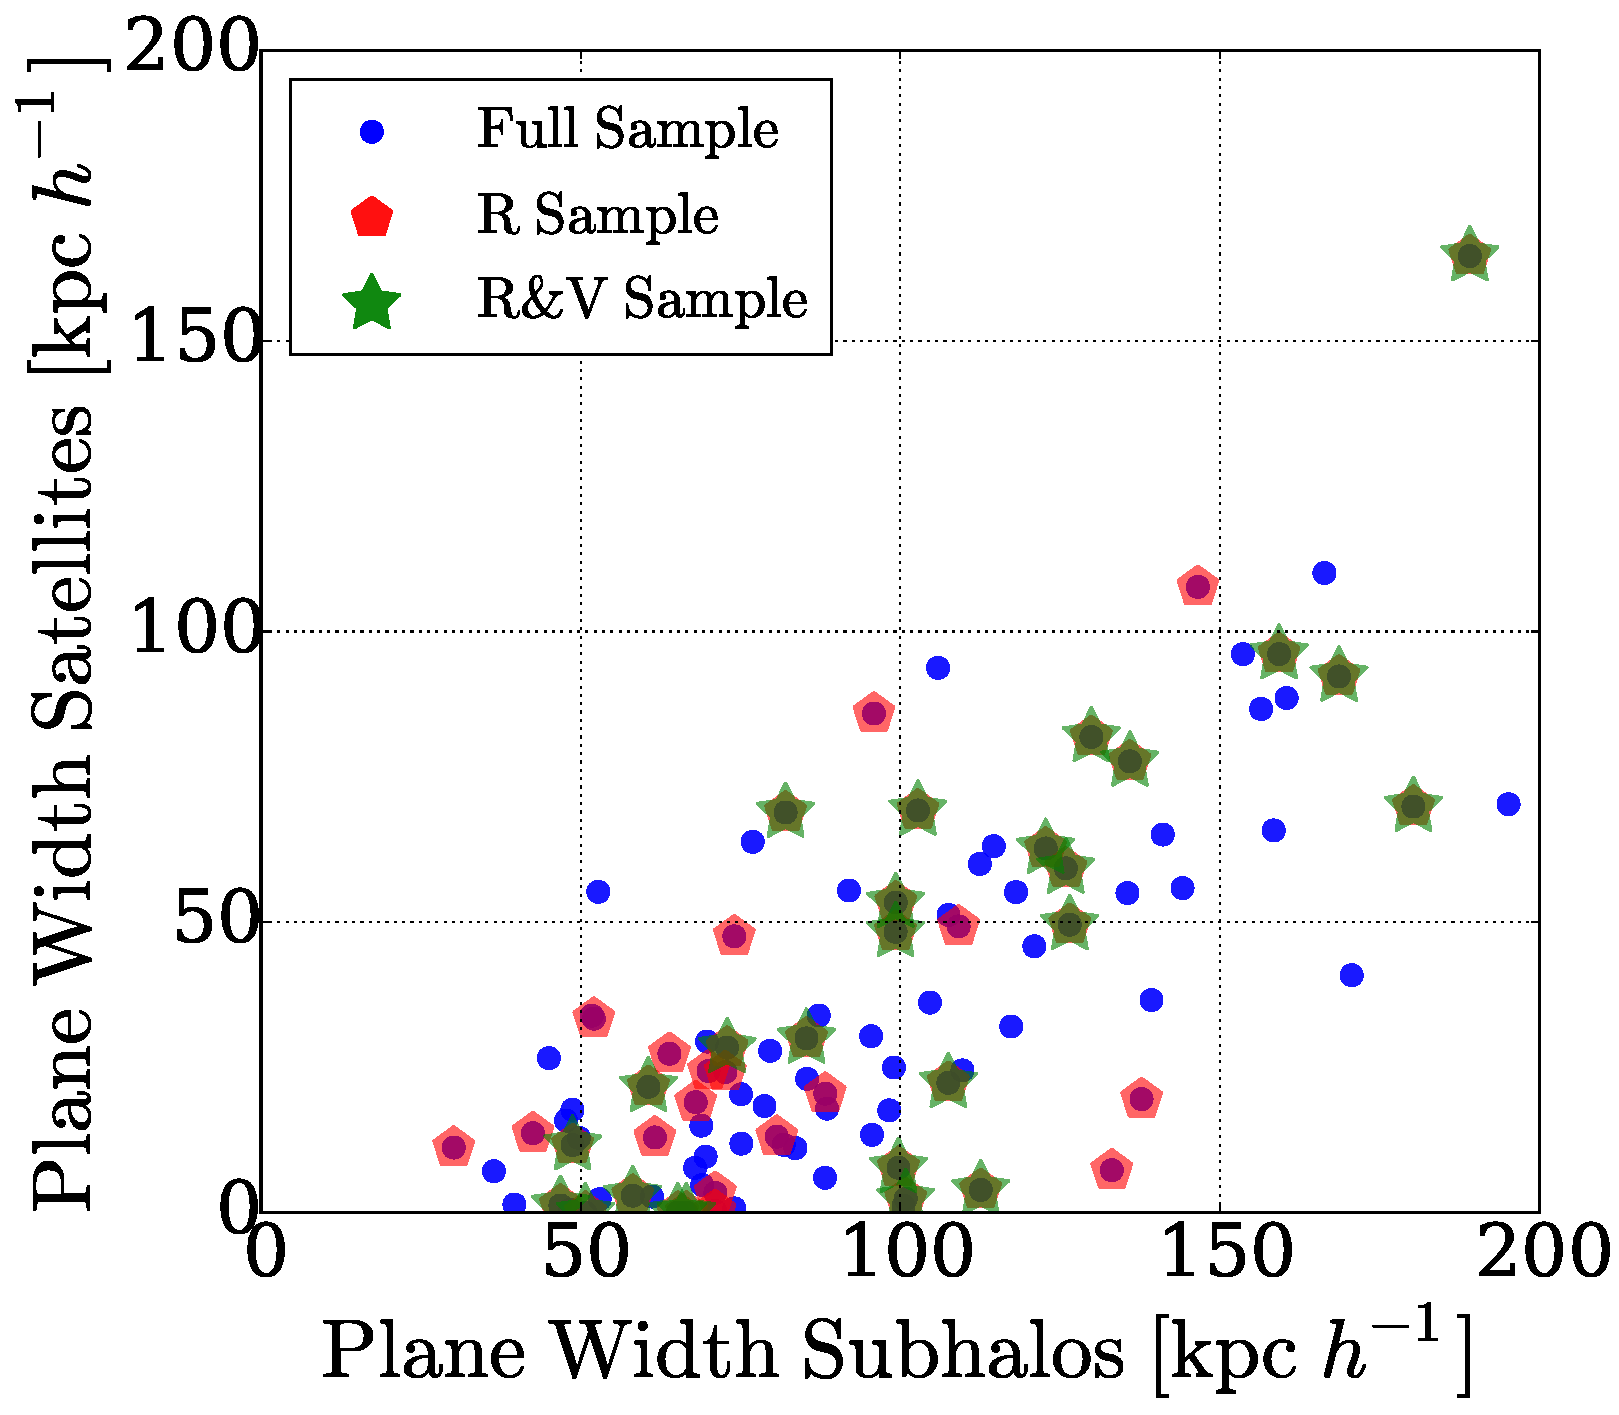
\includegraphics[width=\hsize]{plane_width.pdf}\\
\caption{Plane width for the best planes in the luminious and dark cases.}
\label{fig:plane_width}
\end{figure}

\begin{figure}
\centering
\includegraphics[width=\hsize]{plane_width_n_dark.pdf}\\
\caption{Plane width as a function of objects used to find the plane.}
\label{fig:plane_width_nobjects}
\end{figure}

\section{Results}
\label{Results}

\section{Method}
\label{Method}



%\begin{figure}
%\centering
%\includegraphics[width=\hsize]{Halo_pos_LRomulusRemus.pdf}\\
%\end{figure}

\section{Discussion} 
\section{Acknowledgements}
Gracias.
\bibliographystyle{apj}
\bibliography{Dwarfs}


\end{document}

